\chapter{Xây dựng và triển khai hệ thống}
\label{ch:xay-dung}

\section{Môi trường phát triển}

Hệ thống được phát triển trên Windows với Python 3.x trong môi trường ảo (\texttt{.venv}), quản lý mã bằng Git. Kiểm thử dùng \texttt{pytest}. Đường đánh giá lab không phụ thuộc dịch vụ LLM trực tuyến trả phí, nhằm giữ tính tái lập và kiểm soát chi phí.

\section{Công nghệ và công cụ sử dụng}

\begin{table}[!htbp]
\centering
\caption{Công nghệ, mô hình và công cụ kiểm thử độc lập sử dụng trong đồ án}
\label{tab:tech}
\begin{tabular}{@{}L{0.28\linewidth}L{0.62\linewidth}@{}}
\toprule
\textbf{Thành phần} & \textbf{Lựa chọn} \\
\midrule
Ngôn ngữ \& Môi trường & Python 3.13, Windows 11, NVIDIA GeForce RTX~4050 (6\,GB VRAM) \\
API Gateway & FastAPI / Starlette / Uvicorn \\
Lưu trữ \& Truy hồi lai & SQLite FTS5 (BM25) kết hợp embedding vector \texttt{float32} BLOB + nhân ma trận \texttt{numpy} \\
Kiểm soát truy cập & Pre-retrieval RBAC (tài liệu RAG) + SQLite \texttt{EXPLAIN} \& Authorizer AST (bảng/cột SQL) \\
Mô hình LLM \& Judge cục bộ & Ollama 0.40.11: \texttt{gemma4:e2b-\allowbreak it-\allowbreak q4\_\allowbreak K\_\allowbreak M} (Semantic Judge 2B tối ưu \texttt{think=False}), \texttt{gemma4:e4b-\allowbreak it-\allowbreak qat}, \texttt{qwen3:4b-\allowbreak instruct} (Multi-Tool Agent) và \texttt{claude-\allowbreak sonnet-\allowbreak 5-\allowbreak 5} adapter \\
Giải pháp đối sánh (Baselines) & Meta \texttt{llama-\allowbreak guard3:1b} (Ollama), NVIDIA \texttt{NeMo Guardrails} (\texttt{self\_\allowbreak check\_\allowbreak input} rail) \\
Công cụ \& Benchmark độc lập & NVIDIA \texttt{garak v0.\allowbreak 17.\allowbreak 1} ($2.048$ REST probes), \texttt{PyRIT} Converter \& Adaptive Multi-Turn, HuggingFace \texttt{deepset/\allowbreak prompt-\allowbreak injections} ($662$ mẫu) \\
Kiểm thử tự động & \texttt{pytest} ($469+$ unit \& integration tests trên nhánh hợp nhất) \\
\bottomrule
\end{tabular}
\end{table}

\section{Tổ chức mã nguồn}

Mã nguồn được nhóm theo chức năng để dễ đọc, dễ kiểm thử và tách bạch trách
nhiệm giữa các thành phần. Cụ thể: \texttt{app/} chứa gateway, các guard và
pipeline RAG; \texttt{scripts/} chứa mã sinh dữ liệu và chạy đánh giá;
\texttt{tests/} chứa bộ kiểm thử pytest; \texttt{datasets/} chứa bộ dữ liệu tấn
công và lành tính tổng hợp; \texttt{docs/} lưu tài liệu thiết kế và các quyết
định kỹ thuật. Cách phân tách này giúp thay đổi một lớp guard hoặc một thành phần
truy hồi mà ít ảnh hưởng tới phần còn lại của hệ thống.

\section{Xây dựng chuỗi guard phòng thủ}

Chuỗi guard được hiện thực thành các module độc lập trong \texttt{app/\allowbreak guards/},
mỗi module trả về quyết định trong tập \{Allow, Block, Sanitize, Human-review,
Log\} theo thứ tự mức độ nghiêm trọng cố định (\emph{fail-closed}: quyết định
nghiêm khắc nhất thắng).

\begin{itemize}
    \item \textbf{Input Guard kết hợp Tầng tiền giải mã (\emph{Payload De-obfuscation Pre-decoder}):} Trước khi đối chiếu bộ luật regex, hàm \texttt{\_\allowbreak expand\_\allowbreak deobfuscated\_\allowbreak views()} trong \texttt{app/\allowbreak guards/\allowbreak input\_\allowbreak guard.\allowbreak py} thực hiện chuẩn hoá Unicode NFKC, loại bỏ ký tự ẩn zero-width (\texttt{U+200B..\allowbreak U+FEFF}), gấp đồng hình Cyrillic về Latin, giải nhiễu Leetspeak (\texttt{4->a, 3->e, 1->i, 0->o, 5->s, 7->t}), tự động phát hiện và giải mã các khối Base64 sang UTF-8, cũng như dịch ngược ROT13 khi có tín hiệu mã hoá. Nhờ đó, bộ luật cấu trúc đa ngôn ngữ (Việt/Anh/Đức/Tây Ban Nha) nhìn thấy trực tiếp cả lớp vỏ bọc lẫn mệnh lệnh độc hại ẩn bên trong.
    \item \textbf{RAG Context Guard \& Provenance Guard:} Kiểm tra nguồn gốc tài liệu do máy chủ gán (\texttt{source\_\allowbreak policy.\allowbreak py}) và đối chiếu luật trên từng đoạn ngữ cảnh truy hồi nhằm phát hiện chỉ thị ẩn trong bình luận HTML, giả mạo thẻ hệ thống và mẫu đầu độc kho tri thức; hỗ trợ làm sạch (sanitize) từng đoạn và fail-closed khi bằng chứng tốt nhất bị vô hiệu hoá.
    \item \textbf{SQLite Authorizer AST Guard \& Indirect Result Guard:} Trong \texttt{app/\allowbreak sql\_\allowbreak agent/}, câu lệnh SQL do mô hình sinh ra được kiểm tra bằng \texttt{EXPLAIN} + \texttt{set\_\allowbreak authorizer} trên lược đồ rỗng để cưỡng chế phân quyền tới từng bảng/cột và ép \texttt{LIMIT $\le$ 50}; kết quả trả về từ CSDL tiếp tục được quét từng ô qua \texttt{result\_\allowbreak guard.\allowbreak py} (giải nhiễu gạch nối \texttt{b-ỏ q-u-a}, bắt thẻ \texttt{[INST]}, chặn đổi số tài khoản và che mờ DLP) trước khi đưa vào lần gọi mô hình thứ hai.
    \item \textbf{Output Guard / DLP:} Rà mẫu bí mật (khoá API, JWT, mật khẩu), thông tin định danh cá nhân (PII), liên kết/hình ảnh Markdown thất thoát dữ liệu ra tên miền lạ và mã canary seed từ kho trên phản hồi trước khi trả về người dùng.
    \item \textbf{Semantic Judge cục bộ tối ưu độ trễ (\texttt{gemma4:e2b-\allowbreak it-\allowbreak q4\_\allowbreak K\_\allowbreak M}):} Trong \texttt{app/\allowbreak guards/\allowbreak semantic\_\allowbreak guard.\allowbreak py}, yêu cầu đi qua bộ lọc nhanh (\emph{fast heuristic pre-screen}, $< 0{,}2\,\text{ms}$) và cơ chế \emph{benign short-circuit}; chỉ các truy vấn nằm ở vùng nghi ngờ mới gọi tới mô hình Judge 2B qua Ollama với tham số \texttt{"think": False} và \texttt{num\_\allowbreak predict: 8}, giữ độ trễ mỗi lần gọi Judge ở mức trung vị $\text{p50} = 99{,}79\,\text{ms}$ thay vì hàng nghìn mili-giây như các cấu hình sinh chuỗi suy nghĩ ngầm.
\end{itemize}

\section{Xây dựng cơ chế truy hồi vectorized}

Cơ chế truy hồi lai kết hợp BM25 (SQLite FTS5) với xếp hạng ngữ nghĩa. Để giảm
độ trễ khi kho tài liệu lớn, vector embedding được chuẩn hoá đơn vị và lưu dưới
dạng khối \texttt{float32} (BLOB) trong SQLite; khi truy vấn, toàn bộ ma trận
vector được đọc trực tiếp và chấm điểm bằng \emph{một} phép nhân ma trận
\texttt{numpy} (tích vô hướng chính là cosine do vector đã chuẩn hoá), thay cho
vòng lặp Python và phân tích JSON trên từng tài liệu. Hai danh sách xếp hạng
được hợp nhất bằng Reciprocal Rank Fusion.

Kiểm soát truy cập (RBAC) được áp \emph{trước} bước truy hồi: mỗi tài liệu mang
vai trò/phòng ban và mức nhạy cảm; người dùng chỉ truy hồi được tài liệu trong
phạm vi quyền, độc lập với các guard nội dung.

\begin{figure}[!htbp]
\centering
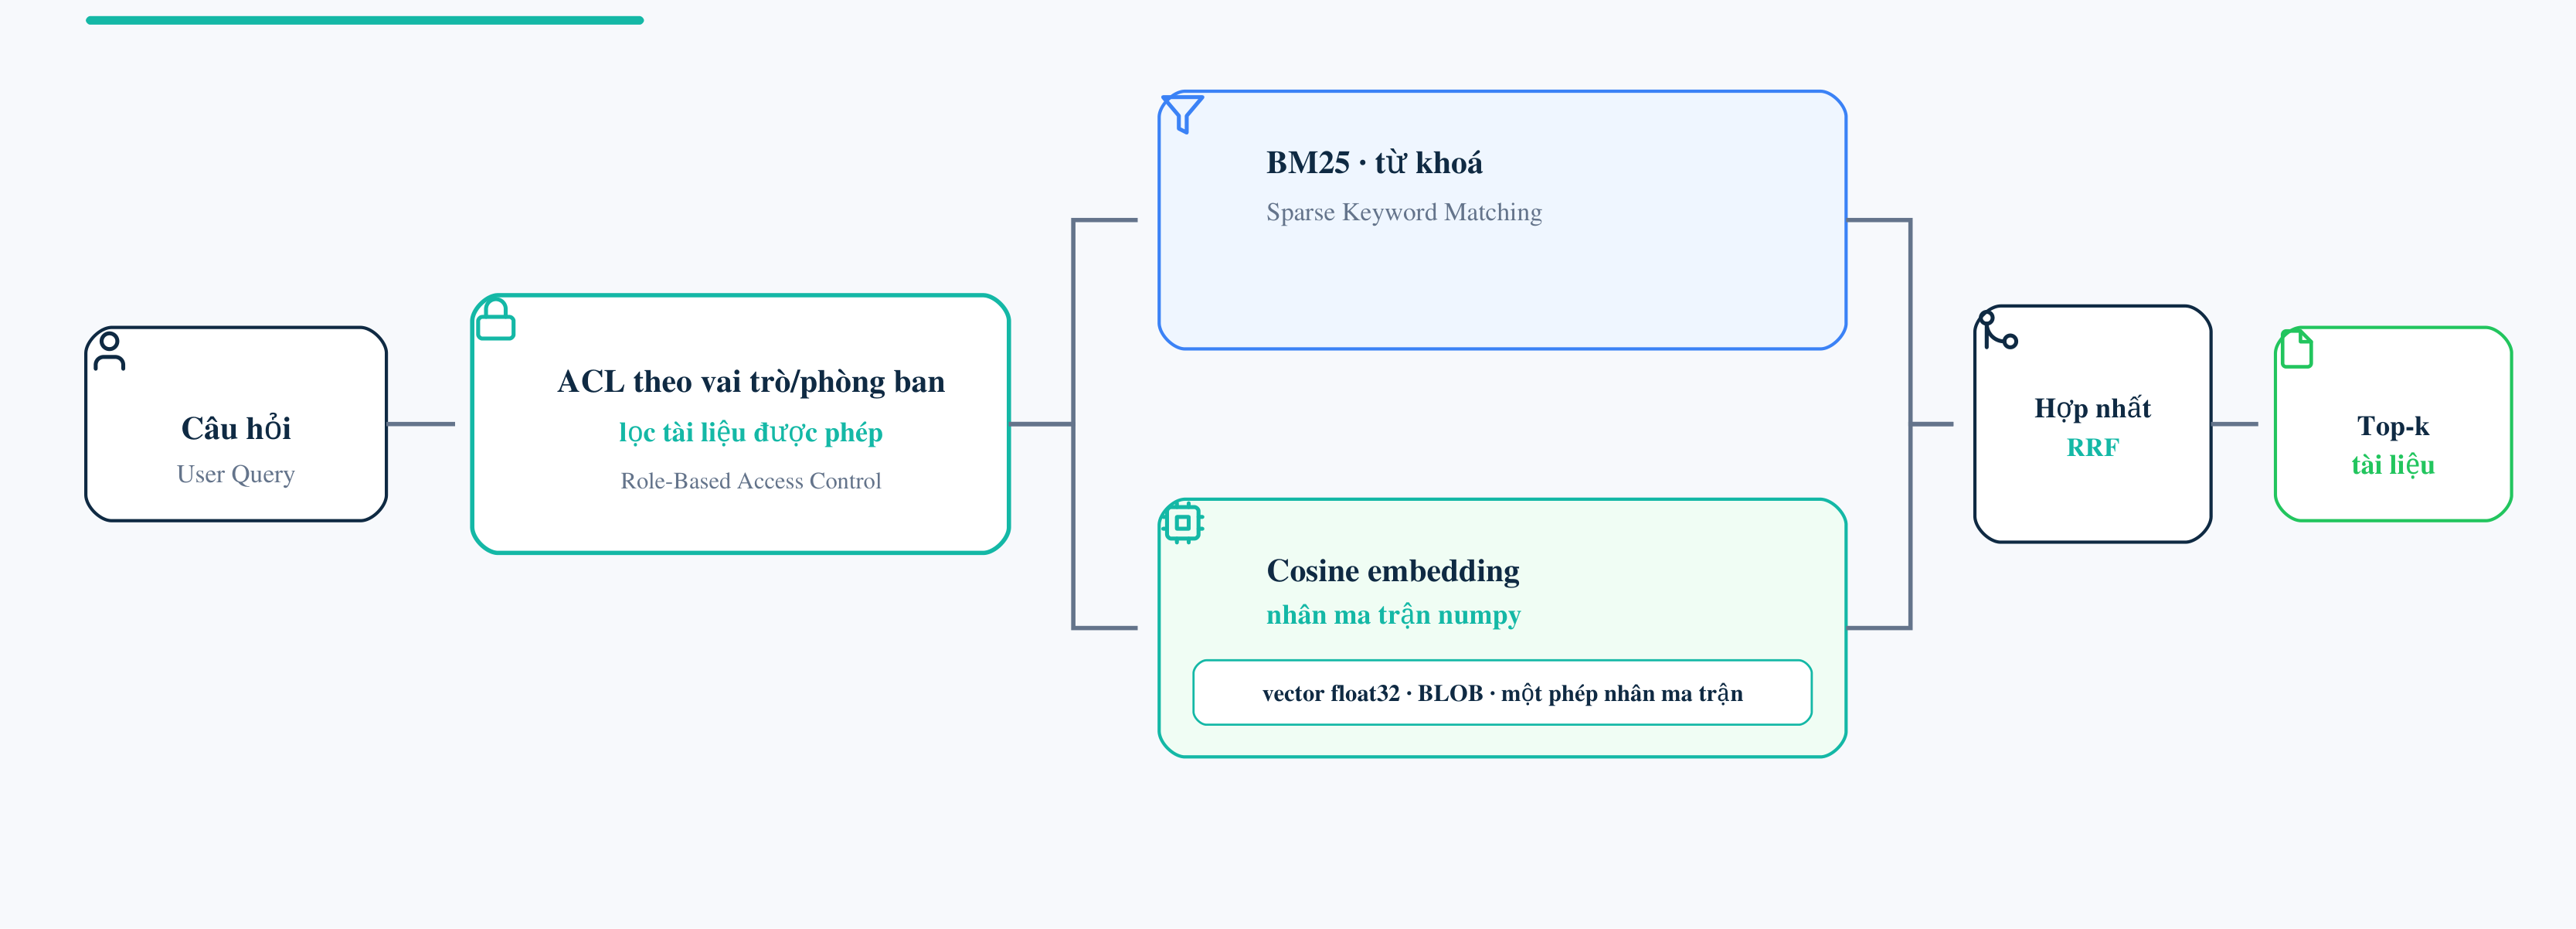
\includegraphics[width=0.78\linewidth]{figures/fig-rag-rbac.png}
\caption{Cơ chế truy hồi lai (BM25 + embedding) kết hợp kiểm soát truy cập RBAC}
\label{fig:rag-rbac}
\end{figure}

Hình~\ref{fig:rag-rbac} minh hoạ luồng: câu hỏi trước hết qua bộ lọc ACL theo
vai trò/phòng ban, sau đó được chấm điểm song song bằng BM25 (từ khoá) và cosine
embedding (nhân ma trận trên vector \texttt{float32}), rồi hai danh sách được hợp
nhất bằng Reciprocal Rank Fusion để chọn ra tài liệu liên quan nhất.

\section{Tích hợp kiểm thử tự động}

Bộ kiểm thử tự động (pytest) bao phủ quyết định của từng guard, pipeline RAG
end-to-end, kiểm soát truy cập RBAC và các kịch bản hồi quy canary/DLP. Mục tiêu
là phát hiện sớm hồi quy khi chỉnh luật hoặc runner, đồng thời giữ bằng chứng
có thể chạy lại trên cùng môi trường lab. Bộ chạy đánh giá ghi kèm provenance
tối thiểu (commit, mô hình, cấu hình, băm dữ liệu) cho các lần chạy mới để truy
vết. Chi tiết kết quả trình bày ở Chương~4.

\section{Kết luận chương}

Chương này trình bày hiện thực chuỗi guard phòng thủ nhiều lớp và cơ chế truy hồi
vectorized kết hợp kiểm soát truy cập RBAC, theo nguyên tắc fail-closed,
content-free và tái lập. Chương~4 trình bày phương pháp và kết quả kiểm thử.
